% kapitel2.tex
\chapter{The ATLAS Detector at the LHC}

\section{The LHC}
The LHC \cite{LHC} is a large hadron and lead nuclei accelerator and collider at CERN, which is a institute located in geneva.
The LHC tunnel has a circumference of around \SI{27}{km}. 
There are detectors placed in several stations of the LHC.
The ATLAS Detector is one of them, but there are further detectors, like CMS, LHCb and ALICE.
In the LHC tunnel both bunches of particles for the collision are accelerated in opposite directions at the same time.
For accelerated protons both bunches can contain up to $10^{11}$ protons.
Therefore each collusion includes many proton-proton collusions.
At each detector there is the possibility to cross the bunches. 
The LHC current reaches a center-of-mass energy of about $\sqrt{s} =$\SI{13}{TeV}. 
High center-of-mass energys are required for producing heavy particles and are therefore essential for a search for vector-like quarks.


\section{The ATLAS Detector}
The ATLAS Detector \cite{ATLAS} is a high luminosity experiment of the LHC. 
The construction of the ATLAS Detector is symmetric around the beam axis with cylindrical components and end caps to cover the full solid angle.
In order to discribe the ATLAS detector a specific coordinate system is selected.
The interaction point is the origin of the coordinate system and the z-axis is parallel to the beam axis, while the x-y plane is perpendicular to the beam axis.
The azimuthal angle $\Phi$ is defined as angle around the beam axis while the polar angle $\Theta$ is measured starting from the beam axis. 
Moreover the pseudorapidity is defined according to $\eta = - \ln(\tan(\nicefrac{\Theta}{2}))$.
With these parameters the distance $\Delta R$ in the pseudorapidity-azimuthal angle space can be calculated with $\Delta R = \sqrt{\Delta \eta^{2} + \Delta \Phi^{2}}$.
Figure \ref{ATLAS} shows the cut-away view of the ATLAS Detector.
\begin{figure}[h!]
\centering
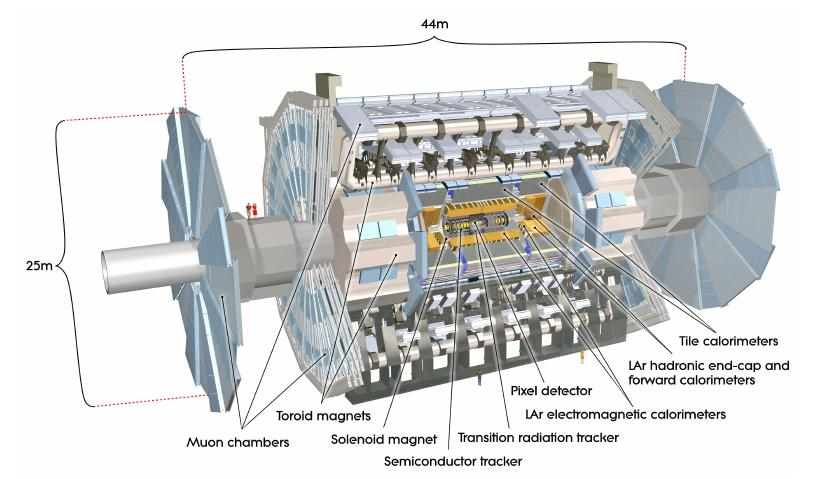
\includegraphics[width=13cm]{figures/atlas.jpg}
\caption{Cut-away view of the ATLAS detector with its different constituents.}
\label{ATLAS}
\end{figure}
There are four main parts the ATLAS detector consists of.
To begin with there is the inner detector, which is the clostest component to the interaction point.
The task of the inner detector is the measurement of vertices and furthermore the measurement of the momenta for all charged particles.
It consits of pixel and silicon microstrip trackers (SCT) and a Transition Radiation Tracker (TRT).
A solenoid magnet surrounds the inner detector and immerses it in a magnetic field with B = \SI{2}{T}. 
This causes the curvature of tracks of charged particles and ensures the momentum measurement.\\
The solenoid magnet is surrounded by the electromagnetic and hadronic calorimeters.
The electromagnetic calorimeter comes first and ensures measurements of electron and photon energies.
Electrons and photons ideally deposit all their energy in the electromagnetic calorimeter by interacting with the detector material.
Other charged particles have also energy depositions in the electromagnetic calorimeter but they are not stopped by the interactions with the detector material. \\
The hadronic calorimeter performs the same goal as the electromagnetic calorimeter for hadrons, which are bound states of the quarks.
Hadrons form jets in the calorimeters.
The particles loose their energy by interacting with the detector material and cause hadronic showers in the hadronic calorimeter.\\
The outermost component of the ATLAS detector is the muon system or muon spectrometer.
For the ideal case only muons reach the muon spectrometer.
The muon spectrometer is immersed with a magnet field resulting from toroid magnets.
The magnets cause the deflection of muons and enable momentum measurements as mentioned for the inner detector.




